\chapter{Pole Cutting Problem}

\section{Descrizione del problema}

Il \textbf{Problema del Taglio delle Aste (Pole Cutting)} può essere
definito nel modo seguente:

\begin{myblockquote}
  Data un'asta di lunghezza $n$ pollici e una tabella di prezzi $p_i$
  per $i = 1, \ldots, n$, \textbf{determinare il ricavo massimo $r_n$ che
    si può ottenere tagliando l'asta e vendendone i pezzi}. Si noti che, se
  il prezzo $p_n$ di un'asta di lunghezza $n$ è sufficientemente
  grande, la soluzione ottima potrebbe essere quella di non effettuare
  alcun taglio.
\end{myblockquote}

\begin{figure}[H]
  \centering
  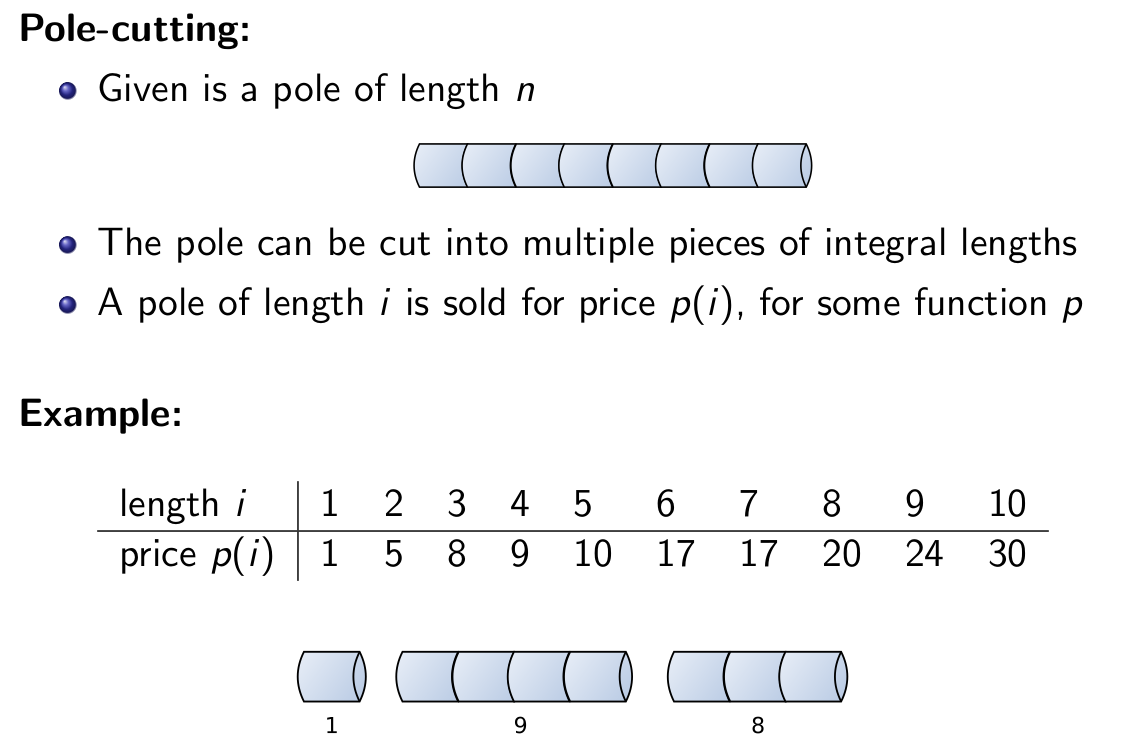
\includegraphics[width=10cm, keepaspectratio]{capitoli/programmazione_dinamica/imgs/pole1.png}
  \caption{La figura mostra un esempio di problema Pole Cutting.}

\end{figure}

\begin{figure}[H]
  \centering
  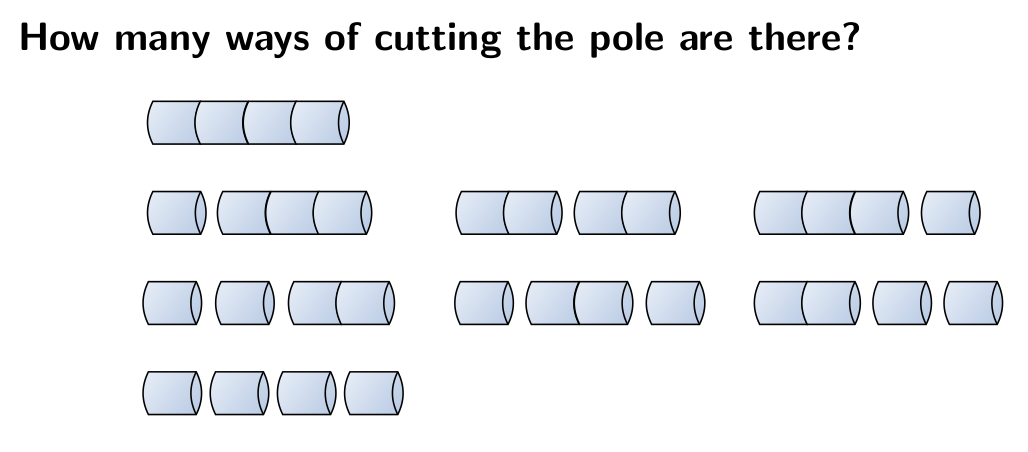
\includegraphics[width=10cm, keepaspectratio]{capitoli/programmazione_dinamica/imgs/pole2.png}
  \caption{La figura sopra invece, mostra tutti i modi in cui può essere
    tagliata un'asta lunga 4 pollici.}
\end{figure}


È importante notare che un'asta di lunghezza $n$ può essere tagliata in
$2^{n-1}$ modi differenti, in quanto \textbf{si ha un'opzione
  indipendente di tagliare o non tagliare}, alla distanza di $i$ pollici
dall'estremità sinistra, per $i = 1, 2, \ldots, n-1$.\\

Se una \textbf{soluzione ottima} prevede il taglio dell'asta in $k$
pezzi, per $1 \le k \le n$, allora una \textbf{decomposizione ottima}
$n = i_1 + i_2, \ldots + i_k$ dell'asta in pezzi di lunghezze
$i_1, i_2, \ldots, i_k$ fornisce il ricavo massimo corrispondente
$r_m = p_{i_1} + p_{i_2} + \ldots + p_{i_k}$

\begin{figure}[H]
  \centering
  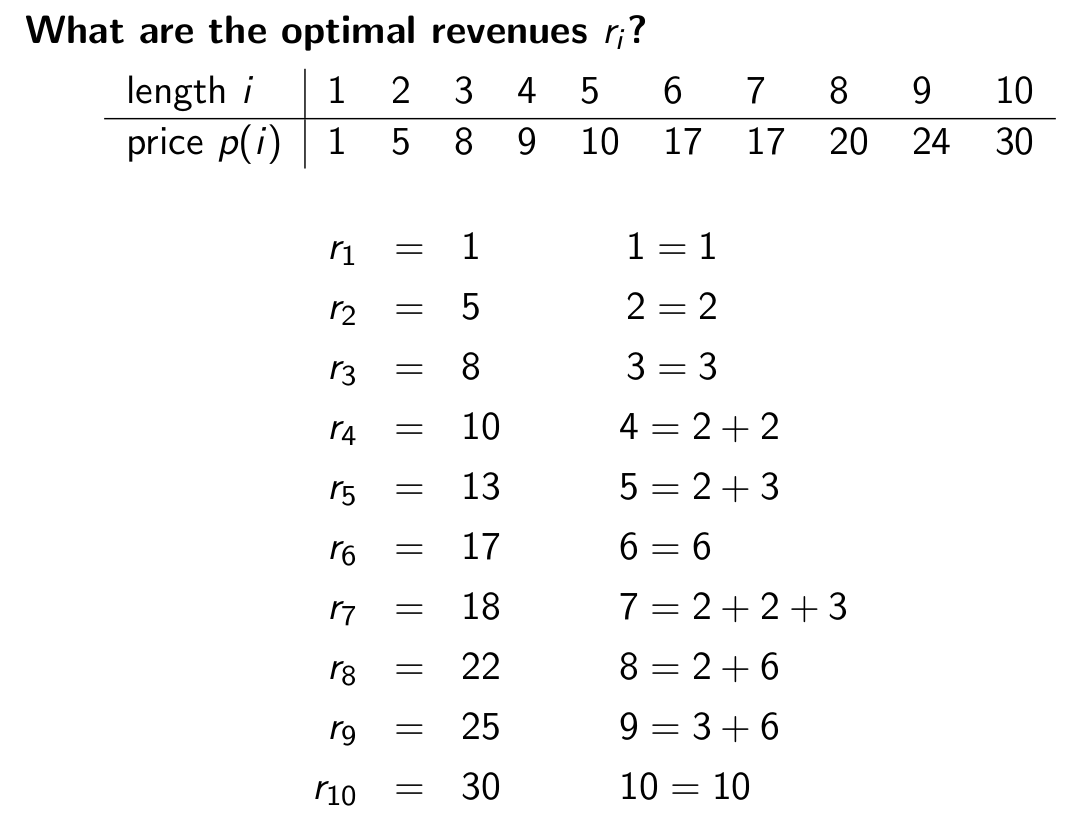
\includegraphics[width=10cm, keepaspectratio]{capitoli/programmazione_dinamica/imgs/pole3.png}
  \caption{Esempio di valori possibili ottenuti tagliando l'asta in vari pezzi}

\end{figure}

\subsection{Goal}

Data un'asta di lunghezza $n$ pollici e una tabella di prezzi $p_i$
per $i = 1, \ldots, n$, \textbf{determinare il ricavo massimo $r_n$ che
  si può ottenere tagliando l'asta e vendendone i pezzi}.

\subsection{Funzionamento}

Più in generale, possiamo esprimere i valori $r_n$ per $n \ge 1$ in
funzione dei ricavi ottimi delle aste più corte:
$$
  r_n = \max(p_n, r_1 + r_{n-1}, r_2 + r_{n-2}, \ldots, r_{n-1} + r_1)
$$

\begin{itemize}
  \item
        Il primo argomento, $p_n$, corrisponde alla vendita dell'asta di
        lunghezza $n$ senza tagli.
  \item
        Gli altri $n-1$ argomenti corrispondono al ricavo massimo ottenuto
        facendo un taglio iniziale dell'asta in due pezzi di dimensione $i$
        e $n-1$, per $i = 1, 2, \ldots, n-1$, e poi tagliando in modo
        ottimale gli ulteriori pezzi, ottenendo i ricavi $r_i$ e $r_{n-1}$
        da questi due pezzi.
\end{itemize}

Per risolvere il problema originale di dimensione $n$,
risolviamo problemi più piccoli dello stesso tipo, ma di dimensioni
inferiori. Una volta effettuato il primo taglio, possiamo considerare i
due pezzi come istanze indipendenti del problema del taglio delle aste.
Possiamo quindi dire che il problema del taglio delle aste presenta una
\textbf{sottostruttura ottima}, ovvero \textbf{le soluzioni ottime di un
  problema incorporano le soluzioni ottime dei sottoproblemi correlati}.\\

Tuttavia, c'è un modo più semplice di definire una struttura ricorsiva
per il problema del taglio delle aste:
\begin{myblockquote}
  Consideriamo la decomposizione formata da un primo pezzo di lunghezza $i$
  tagliato dall'estremità sinistra e dal pezzo restante di destra di lunghezza
  $n-i$. \textbf{Soltanto il pezzo restante di destra (non il primo pezzo) potrà
    essere ulteriormente tagliato}. Possiamo vedere ciascuna decomposizione di
  un'asta di lunghezza $n$ in questo modo: \textbf{un primo pezzo seguito da
    un'eventuale decomposizione del pezzo restante}.  Così facendo, possiamo
  esprimere la soluzione senza alcun taglio dicendo che il primo pezzo ha
  dimensione $i = n$ e ricavo $p_n$ e che il pezzo restante ha dimensione 0 con
  ricavo $r_0 = 0$.
\end{myblockquote}

Otteniamo così la seguente \textbf{versione semplificata
  dell'equazione:}
$$
  r_n = \max_{1 \le i \le n}(p_i + r_{n-i})
$$

Secondo questa formulazione, \textbf{una soluzione ottima incorpora la
  soluzione di un solo sottoproblema} (il pezzo restante) anziché due.

\section{Algoritmo ricorsivo TOP-down}

\begin{lstlisting}[language=Python, mathescape=true]
function Cut-Pole(p, n) {
  Require: Integer n, Array p of length n with prices
  if n == 0 then
    return 0

  $q \leftarrow -\infty$

  for i = 1 $\ldots$ n do
    q $\leftarrow$ max{q, p[i] + Cut-Pole(p, n - i)}

  return q
}
\end{lstlisting}

\subsection{Costo}

Perché questo algoritmo è così \textbf{inefficiente}? Il problema è che
la procedura \texttt{Cut-Pole} chiama più e più volte sè stessa in modo
ricorsivo con gli stessi valori dei parametri, ovvero \textbf{risolve
  ripetutamente gli stessi sottoproblemi}.
\begin{figure}[H]
  \centering
  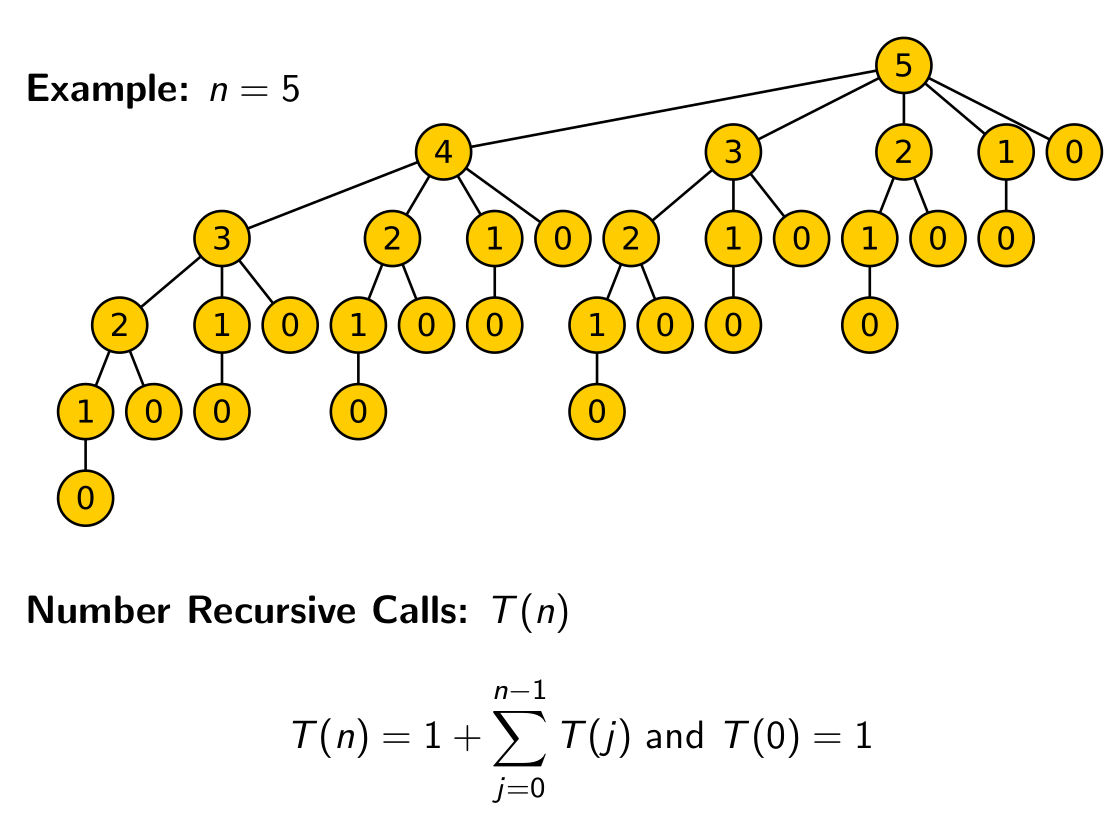
\includegraphics[width=9cm, keepaspectratio]{capitoli/programmazione_dinamica/imgs/pole4.png}
  \caption{Albero delle soluzioni ottenuto da una soluzione trovata con 5 tagli}
\end{figure}

%% TODO: ricontrollare se possibile scrivere tutto su una riga (Tn= sum = 2^n)
$$
  T(n) = 1 + \sum^{n-1}_{j=0}T(j)
$$

$$
  T(n) = 2^n
$$

\paragraph*{Nota:} \texttt{Cut-Pole} è esponenziale in $n$.\\

La procedura \texttt{Cut-Pole} considera esplicitamente tutti i $2^{n-1}$ modi
possibili di tagliare un'asta di lunghezza $n$. L'albero delle
chiamate ricorsive ha $2^{n-1}$ foglie, una per ogni modo possibile di
tagliare l'asta.

\section{Applicare la Programmazione Dinamica al taglio delle aste}

\subsection{Approccio Top-down}

\begin{lstlisting}[language=Python, mathescape=true]
function Memoized-Cut-Pole(p, n) {
  Require: Integer n, Array p of length n with prices

  Let r [0 $\ldots$ n] be a new array

  for i = 0 $\ldots$ n do
    r[i] $\leftarrow$ $-\infty$

  return Memoized-Cut-Pole-Aux(p, n, r )
}
\end{lstlisting}

\begin{lstlisting}[language=Python, mathescape=true]
function Memoized-Cut-Pole-Aux(p, n, r) {
    Require: Integer n, array p of length n with prices, array r of revenues

    if r [n] $\geq$ 0 then
      return r[n]

    if n = 0 then
      q $\leftarrow$ 0
    else
      q $\leftarrow$ $-\infty$
      for i = 1 $\ldots$ n do
        q $\leftarrow$ max{q, p[i] + Memoized-Cut-Pole-Aux(p, n $-$ i, r )}
      r [n] $\leftarrow$ q

    return q
}
\end{lstlisting}

\begin{itemize}
  \item
        Preparare una tabella \texttt{r} di dimensione $n$
  \item
        Inizializza tutti gli elementi di \texttt{r} con $-\infty$
  \item
        Il lavoro effettivo viene svolto in \texttt{Memoized-Cut-Pole-Aux}, la
        tabella \texttt{r} viene passata a \texttt{Memoized-Cut-Pole-Aux}
\end{itemize}

\paragraph*{Nota:} Se \texttt{r{[}n{]}\ $\geq$\ 0} allora \texttt{r{[}n{]}}
\textbf{è stato calcolato in precedenza}

\subsection{Approccio Bottom-up}

\begin{lstlisting}[language=Python, mathescape=true]
function Bottom-Up-Cut-Pole(p, n) {
  Require: Integer n, array p of length n with prices
  Let r[0 $\ldots$ n] be a new array
  r[0] $\leftarrow$ 0

  for j = 1 $\ldots$ n do
    q $\leftarrow$ -$\infty$
    for i = 1 $\ldots$ j do
      q $\leftarrow$ max{q, p[i] + r[j - i]}
    r[j] $\leftarrow$ q

  return r[n]
}
\end{lstlisting}

\subsubsection{Costi}

Il tempo di esecuzione della procedura bottom up è $O(n^2)$, a causa
della doppia struttura annidata del suo ciclo.
$$
  \sum^n_{j=1} \sum^j_{i=1} O(1) = O(1) \sum^n_{j=1} \sum^j_{i=1} 1 = O(1) \sum^n_{j=1} j = O(1) \frac{n(n+1)}{2} = O(n^2)
$$

Anche il tempo di esecuzione della sua \textbf{controparte Top-Down} è
$O(n^2)$, sebbene questo tempo di esecuzione sia un pò più difficile
da spiegare. Poiché \textbf{una chiamata ricorsiva per risolvere un
  sottoproblema precedentemente risolto termina immediatamente}.

\section{Riepilogo}

\begin{itemize}
  \item
        Massimizzare il reward in base ai tagli
  \item
        Tempo di esecuzione dell'approccio Top-Down $O(n^2)$

        \begin{itemize}
          \item
                devo calcolare OPT per ogni $n$, per ognuno pago $n$ \textbf{TEMPO =}
                $O(n^2)$
        \end{itemize}
  \item
        $OPT[j] = \max_{i \le l \le j} (OPT[j-l] + p_l)$
  \item
        salvo i dati in un vettore che contiene $OPT$ dei vari segmenti
        \textbf{SPAZIO =} $O(n)$
  \item
        per ricostruire la soluzione uso un vettore dove $S[j] = \max_l$
        \textbf{SPAZIO\_S =} $O(n)$
\end{itemize}
